\documentclass[11pt]{report}

\usepackage[french]{babel}
\usepackage[utf8]{inputenc}

\usepackage[T1]{fontenc}

\usepackage{tipa}
\usepackage{tipx}

\usepackage{listings}

\title{
\includegraphics[scale=1]{logo.jpg}\\ \textbf{Rapport Finale De Projet Technologique}\\ Traduction de langage SMS\\ 1\up{ère} année}
\author{Réalisé par :\\
		Benjamin Fraquet\\
		Francisco Ruivo\\
		Maël Naccache\\
		Merouane Bousbaa\\\\
		Encadré par :\\
		Nicolas Hernandez}
		
\date{15/05/2013}

\usepackage{graphicx}
\begin{document}

\maketitle

\tableofcontents

\newpage

\begin{center}
\textbf{Résumé}
\newline
Ce projet consiste à transcrire du langage "SMS" vers une phrase française compréhensible.
Ceci a été réalisé au moyen du langage Prolog et de deux approches de traduction : Par dictionnaire et à l'aide de la phonétique.
Le rapport est divisé en deux grandes parties : Le chapitre 2 qui s’intéresse à l'approche théorique du problème et le chapitre 3 qui explique la réalisation technique.
Le premier chapitre introduira rapidement le Prolog et le langage SMS et la dernière partie expliquera l'utilisation du programme ainsi que les améliorations à apporter.
Sur ce, Bonne lecture.
\end{center}

\newpage

\chapter{Introduction}
	\section{Avant-Propos}
	Le sujet de notre projet technologique était la "Traduction de langage sms/chat/forum en francais". La seule contrainte était de réaliser le projet en Prolog via l'implémentation libre SWI-Prolog. Si vous vous posez la question de ce qu'est le langage SMS ou ce qu'est Prolog, référez-vous respectivement aux sections 1.2 et 1.3. Ce qu'il faut brièvement comprendre c'est qu'il nous était demandé de traduire un ensemble d'abréviations françaises vers une phrase compréhensible pour le commun des mortels. Nous devions donc créer une petite intelligence artificielle capable de faire ceci pour nous. Pour cela, plusieurs idées nous sont venues à l'esprit, elle seront abordées dans la section 1.4.
	\paragraph{} Sur ses mots, je vais vous laisser l'immense joie de consulter le reste de ce rapport afin de découvrir le magnifique univers de la traduction, vu par des étudiants en première année. Une expérience qui, je n'en doute point, ne manquera pas de vous surprendre ( en bien ou en mal, je ne garantis rien ).
	
	\section{Du langage SMS}
	Vous l'avez déjà sûrement rencontré, que ce soit par vos enfants, vos neveux, voire peut-être même vos élèves, il y a peu de chances que vous y ayez échappé. Prenant la forme de messages très courts et rarement compréhensibles pour les non-initiés, le langage SMS à pour origine, comme son nom l'indique, le SMS.
	\paragraph{}
	SMS est l'abréviation de {\em Short Message Service}\footnote{Source: wikipedia.org/wiki/Short\_Message\_Service} ( Comme l'on dirais en Anglais de spécialité ). Il fait partie de la norme GSM et fut développé dans les années 1980, toutefois, son ouverture au grand public date des années 2000. Historiquement, pour des raisons techniques, la taille d'un SMS a dû être limitée à 128 octets, c'est à dire, environ 146 caractère ASCII 7bits. Il faut de plus noter que les forfaits proposant des SMS illimités par les opérateurs grands public sont relativement récents ( on commence à en voir apparaître en 2004 mais ceux-ci sont souvent limités au réseau de l'opérateur et coûteux\footnote{Exemple du premier forfait "Illimité" de Bouygues Telecom : lesmobiles.com/actualite/1453-bouygues-lance-le-premier-forfait-sms-illimite.html} ). Aussi, l'utilisation d'abréviations dans les SMS s'est démocratisée afin de pouvoir transmettre un maximum d'information pour un coût minimal.\\
	De plus, un autre facteur s'est rajouté à ceci : l'agencement E.161 utilisé dans la plupart des téléphones portables. En effet, il était relativement difficile d'embarquer un clavier classique à 102 touches tout en restant portable. Toutefois, cet agencement a plusieurs défaut : Il rend l'écriture plus longue, rend difficile d'accès les caractères accentués et spéciaux ( tel que l'apostrophe ) ainsi que les majuscules. Cela a pour conséquence une utilisation à outrance des abréviations, la suppression des accents et autres caractères spéciaux ( qui de plus étaient bien souvent codés sur 1 octet ou plus au lieu de 7 bits, ce qui limitait d'autant plus la taille du SMS ) et utilisation de toute autre méthode pouvant réduire le temps de frappe et la taille du message.\\
	Le langage SMS était né.\\
	Malgré l'invention de l'aide à la frappe ( tel que le T9\footnote{wikipedia.org/wiki/Text\_on\_9\_keys\#T9} ) et la généralisation des forfaits dits "illimités", le langage SMS continue toujours à être utilisé, notamment sur internet, puisqu'il permet de communiquer un message écrit en un minimum de temps et d'effort, au détriment de la qualité du dit message et du respect du récepteur qui aura bien souvent du mal à déchiffrer le message.\\
	Voici un exemple\footnote{Merci à Mr. Batiste Martin du Groupe 4 qui m'aura fournit cet exemple.} : \\
	\indent {\em slt comen sa va t ou y fo kon se voa}\\
	Que l'on traduirait par :\\
	\indent {\em Salut. Comment ça va ? Tu es ou ? Il faut que l'on se voit.}\\\\
	Vous serez vous même juges de la compréhensibilité de ce message.\\
	Nous allons désormais voir un autre langage, plus vieux que le SMS et surtout, plus formel.
	
	\section{De Prolog}
	Prolog, pour PROgrammation LOGique, fut conçu en 1972 par Alain Colmerauer et Philippe Roussel à l'Université d'Aix-Marseille. Bien que l'on trouve des langages utilisant principalement la logique plus anciens que Prolog ( Absys ou Planner en 1969 ), Prolog est le premier langage à réellement utiliser le paradigme de programmation logique.\\
	Prolog est un langage interprété, toutefois, il fonctionne différemment de ce que l'on voit chez Python, PHP, et autre langage interprété. En effet, en Prolog, l'interpréteur n'est pas là pour exécuter un programme, il est là pour apprendre et pour répondre à des questions. En effet, lorsque l'on code en Prolog on va en vérité créer des faits et des règles qui seront vrais si ils peuvent s'unifier et faux sinon et on va les apprendre à notre interpréteur, on lui posera ensuite des questions sur ces faits et règles, et l'interpréteur nous répondra s'ils sont vrais ou faux en fonction de ce qu'on lui aura appris. Il peut même, grâce au mécanisme d'unification, chercher pour une seule question, toutes les réponses vraies.\\
	Il est compliqué de comprendre comment on peut programmer ainsi, toutefois, tout sera expliqué dans le Chapitre 3 et la section 4.1.
	
	\section{Avant de programmer, des idées !}
	Si vous ne le saviez déjà pas, vous devriez avoir désormais une vague idée de ce qu'est le langage SMS et le Prolog. Bien. Mais revenons au cœur du sujet : Comment allons nous traduire du SMS vers un français plus ou moins correct ?
	\paragraph{}
	Deux grandes idées nous sont venues en tête. La première est relativement simple, il suffit de créer un dictionnaire de correspondance à la manière d'un dictionnaire français-anglais, par exemple. Il nous suffirait d'apprendre à notre petite intelligence artificielle la signification de chaque acronyme SMS pour qu'elle puisse traduire une phrase mot-à-mot.\\
	La seconde idée est de se baser sur la phonétique des mots. En effet, en SMS certains mots changent de forme mais pas de prononciation par exemple {\em Comment} peut s'écrire {\em komen} mais se prononcera toujours /\textipa{k\!Om\~a}/, on peut ainsi "deviner" la signification de certains mots.
	\paragraph{}
	Nous allons étudier ces idées plus en détails dans le chapitre suivant.

\chapter{Partie Théorique}
	\section{Posons quelques axiomes}
	Avant d'expliquer notre démarche, il nous faut poser quelque axiomes que nous utiliserons dans notre traduction et expliquer pourquoi nous avons fait ces choix d'axiomes.\\
	Les voici : \\
	\begin{itemize}
		\item \textbf{1 - Le SMS ne change pas l'ordre des mots et de la ponctuation dans la phrase.}\\
		Le langage SMS n'est qu'un ensemble d'abréviations, aussi, il n'est pas sensé pouvoir changer la position d'un mot dans une phrase. Nous sommes d'accord que {\em J'aime les patates.} et {\em J'patates. les aime} n'ont pas la même signification, aussi {\em jm lé patat} et {\em jpatat lé m} sont tout autant différents.\\
		
		\item \textbf{2 - La traduction peut être ambigue}\\
		La traduction n'est pas une fonction, par là nous voulons dire qu'une même abréviation peut être traduite en plusieurs mots différents. Un exemple simple sont les conjugaisons de verbes : {\em komenc} pourrait se traduire par {\em commencer}, {\em commencé} ou encore {\em commencez}.\\
		
		\item \textbf{3 - Un mot en SMS peut être traduit par un groupe de mots}\\
		Par exemple, {\em c.à.d} veut dire {\em C'est à dire}.\\
		
		\item \textbf{4 - Un mot est encadré par deux espaces}\\
		C'est cette définition d'un mot que nous choisissons pour notre traduction. Elle vous aura sûrement choqué au plus profond de votre petit cœur sensible. En effet, {\em J'étais} est constitué de deux mots, or, selon notre définition, {\em J'étais} n'est qu'un mot. Alors, pourquoi cette hérésie ? Si vous avez bien lu la section 1.2, vous avez peut-être déjà une petite idée. Rappelez-vous, nous avons parlé de l'agencement E.161 qui rendait difficile d'accès les caractères spéciaux, dont l'apostrophe et toute autre ponctuation. Aussi, il est relativement sûr d'assumer qu'une phrase SMS ne contiendra ni apostrophe, ni ponctuation autre que point d'exclamation ou d'interrogation ( en vérité, il s'agit plus souvent de $ \forall n \in [5;+\infty] | n \times ? \vee n \times ! $ ). Toutefois, nous allons tout de même traiter la ponctuation comme des mots, seules les apostrophes ne seront pas traitées.\\
		\item \textbf{5 - Une phrase en SMS est entièrement en minuscules}\\
		Cet axiome est nécessaire dû à un détail technique que nous expliquerons dans le Chapitre 3. Il peut se justifier pour les mêmes raisons que l'axiome ci-dessus.\\
	\end{itemize}
	
	Nous voila désormais armés pour entamer nos traductions !
	
	\section{Larousse mon amour}
	Nous allons donc mettre en œuvre une traduction par dictionnaire. L'avantage de ce type de traduction est sa simplicité de mise en œuvre, sa rapidité et, dans le cas de langages que l'on peut traduire littéralement Mot-à-Mot comme le SMS, sa traduction quasi-parfaite s'il n'y à pas d'ambiguïtés. Pour cela, il nous faut juste créer une "base de connaissances" ( on peut voir cela comme une base de données relationnelle ) mettant en relation pour chaque abréviation SMS, le ou les mots français lui correspondant. Une fois que notre intelligence artificielle a pris connaissance de cette base, il lui suffit de "découper" une phrase mot à mot, selon l'axiome 4, et de traduire chacun d'entre eux grâce à sa base de connaissances.
	\paragraph{}
	Cette méthode a toutefois de gros défauts : Elle ne peut traduire un mot si il n'est pas dans sa base de connaissances, ne peut déterminer la traduction la plus probable dans le cas d'ambiguïtés, et nécessite de créer une énorme base de connaissances qui va devoir régulièrement changer. De plus, elle est incapable de s'adapter à des mots polymorphes en dehors de connaître leurs très nombreuses itérations.\\
	En bref, on ne peut se contenter de cette méthode et il nous faut trouver un autre moyen de traduction.
	
	\section{Super-phonétique à la rescousse !}
	Nous l'avons déjà abordé dans la section 1.4, nous pouvons utiliser la phonétique des mots pour les traduire.
	La mise en œuvre de cette méthode est légèrement plus compliquée : Elle nécessite de connaître tous les phonèmes de la langue française et de savoir découper un mot en tout ses phonèmes. Toutefois, une fois cette étape faite, le reste s'avère relativement simple : Une fois le mot SMS traduit en son équivalent phonétique on va rechercher si on peut l'unifier avec un mot français lui même traduit en phonétique, si oui, alors il s'agit très probablement de sa traduction.
	\paragraph{} Notez comment j'ai précisé "probablement" dans la phrase précédente. Et bien oui, la méthode par la phonétique n'est malheureusement pas parfaite. Si elle à l'avantage de traduire sans problèmes les mots polymorphes ( pour elle {\em komen}, {\em comen}, {\em coman}, etc ... sont équivalents ), il n'est pas garanti qu'elle fournisse une bonne traduction ( un mot en SMS peut avoir la même phonétique qu'un mot français sans être ce mot ) et, de plus, une simple modification de la phonétique entre l'abréviation et sa traduction réelle, bien que négligeable par l'oreille humaine ( par exemple /\textipa{\~a}/ et /\textipa{\~O}/ sont relativement similaires ) fera rater la traduction par cette méthode.\\
	Nous avons donc opté pour une solution prenant en compte les avantages et défauts de chaque méthode.
	
	\section{Passons le tout au mixeur}
	Nous avons donc décidé d'utiliser les deux méthodes dans un ordre bien défini. Tout d'abord, on essaye de traduire la phrase via l'approche par dictionnaire et ensuite on utilise l'approche phonétique pour tous les mots que nous n'avons pu traduire précédemment. Faire ainsi a l'avantage de permettre de garder une base de connaissances relativement réduite, mais sûre, pour l'approche par dictionnaire, permettant donc une traduction relativement fidèle, et de garder les mots variants pour l'approche par phonétique qui est plus adaptée.\\
	Cette méthode n'est bien sûr pas non plus exempt de défauts, toutefois, nous aborderons ceci dans la section 4.3 dans laquelle nous aborderons aussi les solutions techniques et théoriques à tous les problèmes que nous avons pu rencontrer.

\chapter{Partie Technique}
Cette partie va se concentrer sur l'implémentation des idées proposées dans le Chapitre 2. Elle présentera aussi les différents problèmes techniques rencontrés lors de la réalisation du projet.

	\section{Un peu de dictionnaire dans mon Prolog}
	Avant d'essayer d'implémenter un dictionnaire en Prolog, essayons de modéliser ce que représente un dictionnaire.\\
	Nous pouvons voir un dictionnaire Français-SMS comme un ensemble de relations entre différents éléments ( ici, les mots ). Très simplement nous pouvons écrire ceci comme :\\
	\smallskip
	
		$ 
			Dictionnaire \in \{ \\
			\indent	"bjr" \rightarrow "bonjour"\\
			\indent "slt" \rightarrow "salut"\\
			\indent \}
		$\\
	
	\noindent Cette association d'élèment se retrouve dans la plupart des langages sous la forme des tables de hachages. Toutefois, Prolog ne dispose pas de ce type de donnée, mais, du à la nature logique du langage, il est aisé de créer ce type de relation.\\
	Nous avons donc choisi d'utiliser les \emph{Faits} pour implémenter ceci. Un dictionnaire peut s'exprimer sous la forme d'un fait d'arité 2 comprenant un mot SMS et son équivalent Français. L'équivalent de l'écriture relationnelle précédente s'écrit donc en Prolog :\\
	
	\begin{lstlisting}[language=Prolog]
	dico('bjr','bonjour').
	dico('slt','salut').
	\end{lstlisting}
	
	Nous avons donc créer une première base de connaissances pour notre intelligence artificielle. Ainsi, nous pouvons déjà commencer à traduire grâce à l’interpréteur Prolog, par exemple, pour traduire {\em "bjr"} :
	\begin{lstlisting}[language=Prolog]
	?- dico('bjr',E).
	E = 'bonjour'.
	
	true.
	\end{lstlisting}
	
	Nous avons donc une première traduction par dictionnaire fonctionnelle, toutefois celle-ci n'est pas très pratique à utiliser et ne traduit qu'un mot à la fois. Comment allons nous faire pour traduire des phrases ?\\
	Pour cela nous allons utiliser une {\em Règle}. Sans faire un cours de Prolog ( ce qui n'est pas le but de ce rapport et qui est hors de mes compétences ), une règle est simplement un terme complexe composé d'autres règles et de faits que l’interpréteur Prolog va chercher à unifier.
	\paragraph{}
	Nous pouvons donc écrire une règle récursive qui va parcourir une liste de mots en SMS en séparant la tête de la liste et la queue de la liste, va appliquer le fait {\em dico/2} sur la tête, placer le résultat dans la tête de la liste en second argument puis passer les queues des deux listes à elle même pour ainsi traduire toute la liste jusqu'à la fin :
	
	\begin{lstlisting}[language=Prolog]
	smsVersFr([],[]). % Cas final.
	smsVersFr([Tete|Queue],[Tres|Qres]) :-
		dico(Tete,Tres),  
		smsVersFr(Queue,Qres).
	\end{lstlisting}
	
	Cette règle nous permet donc de traduire une liste d'atomes ( Ici représentant des mots en SMS ) littéralement mot-à-mot. Par exemple :
	
	\begin{lstlisting}[language=Prolog]
	?- smsVersFr(['slt','bjr'],E). 
	E = [salut, bonjour].
	
	true.
	\end{lstlisting}
	
	Nous pouvons encore améliorer ce système en créant une règle prenant une chaîne de caractères et renvoyant les traductions trouvées. Pour cela, il nous suffit de découper la chaîne en liste d'atomes. Il existe une règle de SWI-Prolog permettant ceci, il s'agit de {\em atomic\_list\_concat/3}. Cette règle a trois arguments : Une liste d'atomes, une chaîne qui servira de séparateur et la chaîne à découper. Nous utilisons un espace comme séparateur. Ce choix est dû à l'Axiome 4, ce qui simplifie le système mais a pour principal défaut de ne pas gérer la ponctuation, par exemple, si l'on cherche à découper la phrase {\em "bjr, slt"} nous obtiendrons les atomes {\em ['bjr,', 'slt']}. {\em 'bjr,'} sera donc consiéré comme un mot, hors, notre dictionnaire connais {\em "bjr"} mais pas {\em "bjr\textbf{,}"}, cela empêchera donc la traduction. Nous expliquerons plus tard comment nous avons résolu ce problème. Pour le moment nous devons faire avec.\\
	La règle de découpage est donc simple à écrire :
	
	\begin{lstlisting}[language=Prolog]
	chaineVersAtom(Chaine, ListeAtom) :-
		atomic_list_concat(ListeAtom, ' ', Chaine).
	\end{lstlisting}
	
	Par exemple :
	
	\begin{lstlisting}[language=Prolog]
	?- chaineVersAtom('bjr slt', B).
	B = [bjr, slt].
	
	true.
	\end{lstlisting}
	
	Il nous suffit ensuite de créer une règle utilisant les règles précédentes pour traduire une chaine de caractères :
	
	\begin{lstlisting}[language=Prolog]
	traduire(Sms, Fr) :-
		chaineVersAtom(Sms, Liste),
		smsVersFr(Liste, Fr).
	\end{lstlisting}
	
	Ce qui nous donnera :
	
	\begin{lstlisting}[language=Prolog]
	?- traduire('bjr slt',E).
	E = ['bonjour', 'salut'].
	
	true.
	\end{lstlisting}
	
	Nous avons donc une traduction par dictionnaire fonctionnelle et simple d'utilisation. Une seule chose reste à régler : Que se passe-t-il si nous donnons à notre intelligence artificielle un mot qui n'est pas dans sa base de connaisances ?
	
	\begin{lstlisting}[language=Prolog]
	?- traduire('bjr lol',E).
	false.
	\end{lstlisting}
	
	{\em "lol"} n'étant pas dans sa base de connaissances, il ne peut unifier {\em dico('lol',X).} et répond donc que la requête est fausse.\\
	Nous pouvons forcer l'intelligence artificielle à traduire quand bien même elle ne connait pas le mot simplement en utilisant le fait {\em dico(X,X).}. Ce fait associera tout mot à lui même. Il doit être déclaré après toutes les autres occurrences de dictionnaire ( autrement tout mot sera remplacé par ... lui même, ce qui n'est pas très intéressant ). En ajoutant ce fait on obtient donc :
	
	\begin{lstlisting}[language=Prolog]
	?- traduire('bjr lol',E).
	E = ['bonjour','lol'].
	
	true.
	\end{lstlisting}
	
	Ce comportement n'est pas forcément désirable puisque la traduction est de ce fait faussée mais cela permet à l'IA de fonctionner malgré tout.
	La traduction par dictionnaire est donc utilisable, la plus grande difficulté ici étant de créer une base de faits suffisamment grande pour traduire le plus de termes possibles.\\
	Toutefois, nous avons encore le problème d'être incapable de traduire les mots inconnus, pour cela nous avons développé une deuxième traduction.
	
	\section{Une /so.ly.sj\textipa{\~O}/ différente}
	Quel est le point commun entre {\em Comment}, {\em Komen} et {\em coman} ?\\
	Ils se prononcent de la même manière ! En effet, les 3 se traduisent par /\textipa{kOm\~a}/ en phonétique. Si nous arrivions à traduire les mots en SMS en phonétique, nous pourrions les comparer à une base connue de mots et ainsi trouver les traductions possibles du mot.\\
	Nous allons tout d'abord nous intéresser à la traduction d'un mot en SMS. Pour cela nous nous basons sur le système API Français pour avoir la liste des phonèmes\footnote{Source : https://en.wikipedia.org/wiki/Help:IPA\_for\_French}. Il nous faut donc créer une base de connaissances contenant ces phonèmes. Pour cela nous avons utilisé un script Ruby pour parser la syntaxe de la page wikipedia, les fichiers ruby et les regexp utilisés sont disponibles dans le dossier v2.0/ à la racine du projet.
	Nous avons donc créé un ensemble de faits dont voici certains exemples :\\
	
	\indent phon([99,104],'\textipa{k}').\\
	\indent phon([114],'\textipa{K}').\\
	\indent phon([114,104],'\textipa{K}').\\
	\indent phon([99,104],'\textipa{\:l}').\\
	\indent phon([115,99,104],'\textipa{\:l}').\\
	
	Vous vous demandez peut-être ce que représente la liste en premier argument. En vérité, nous avons légèrement ( mais vraiment légèrement, et puis c'était pour votre bien d'abord ) menti quand nous vous avions présenté {\em 'slt bjr'.} comme étant une chaine. En vérité, en Prolog, toute chaîne écrite entre apostrophe est un atome. Une chaîne est en fait une liste de nombre représentant le caractère en UTF-8 \& ASCII 7bits en base 10. Ici, puisque nous allons traiter les mots caractère par caractère il est important de traiter des vraies "Chaînes", auquel cas nous traiterions atomes par atomes, ce que nous ne souhaitons pas. Donc, cette base de connaissances pourrait se lire :\\
	
	\indent phon('ch','\textipa{k}').\\
	\indent phon('r','\textipa{K}').\\
	\indent phon('rh','\textipa{K}').\\
	\indent phon('ch','\textipa{\:l}').\\
	\indent phon('sch','\textipa{\:l}').\\
	
	Bien, maintenant, comment convertir un mot en son équivalent phonétique ? Tout d'abord il faut le convertir en chaîne. Cela se fait via la règle name/2 de Prolog :
	
	\begin{lstlisting}[language=Prolog]
	?- name('Bonjour !',E). 
	E = [66, 111, 110, 106, 111, 117, 114, 32, 33].
	
	true.
	\end{lstlisting}
	
	Une fois ceci fait, il faut simplement convertir les caractères en phonèmes grâce au fait {\em phon/2} toutefois nous avons un problème. En effet, tous les phonèmes ne sont pas composés d'un même nombre de caractères, par exemple nous avons vu dans notre base de connaisances que {\em r = \textipa{K}} ( 1 lettre = 1 phonème ) mais aussi que {\em rh = \textipa{K}} ( 2 lettres = 1 phonème ). Comment faire pour gérer cela ?\\
	Et bien cela est simple puisque les listes en Prolog sont {\em magiques}. Vous vous rappelez peut-être de la notation {\em [T|Q]} que nous avons utilisé dans la traduction par dictionnaire pour obtenir la tête et la queue d'une liste ? Et bien il est tout à fait possible d'écrire {\em [T1,T2,...,Tn|Q]} pour récupérer n élément en tête de liste.\\
	Sachant qu'un phonème en français n'est pas composé de plus de 3 lettres, nous avons juste à dériver la règle de traduction en 3 variantes : une prenant 1 lettre, une en prenant 2 et une dernière en prenant 3.\\ 
	La règle est très similaire à la règle smsVersFr/2 vue dans la traduction par dictionnaire. Elle prend 2 listes en arguments, applique un fait sur la ou les têtes de la 1\up{ère} liste, la place dans la tête de la 2\up{ème} liste puis s'applique récursivement sur les queues des listes :
	
	\begin{lstlisting}[language=Prolog]
	getPhon([],[]).
	getPhon([T1,T2,T3|R],[H|Q]) :- phon([T1,T2,T3],H), getPhon(R,Q).
	getPhon([T1,T2|R],[H|Q]) :- phon([T1,T2], H), getPhon(R,Q).
	getPhon([T1|R],[H|Q]) :- phon([T1],H), getPhon(R,Q).
	\end{lstlisting}
	
	Ainsi, si nous essayons de traduire {\em Chat} en phonétique nous écrivons :
	\begin{lstlisting}[language=Prolog]
	?- name('chat',X), getPhon(X,B).
	\end{lstlisting}
	\indent \indent \indent \indent X = [99, 104, 97, 116],\\
	\indent \indent \indent B = [\textipa{\:l}, a, s] ;\\
	\indent \indent \indent X = [99, 104, 97, 116],\\
	\indent \indent \indent B = [\textipa{\:l}, a, t] ;\\
	\indent \indent \indent X = [99, 104, 97, 116],\\
	\indent \indent \indent B = [\textipa{\:l}, \textipa{A}, t].\\
	\begin{lstlisting}[language=Prolog]
	true.
	\end{lstlisting}
	
	Prolog va générer toute les traductions possibles grâce à sa base de connaissances. Nous pouvons noter qu'elles ne sont pas toutes entièrement fidèles au mot toutefois, nous avons fait le choix de garder cette approximation car nous cherchons à traduire en phonétique du SMS, qui lui n'est pas forcément fidèle au mot d'origine non plus.\\
	Cette marge d'approximation permet ainsi d'augmenter les traductions possibles et donc la probabilité de générer une traduction que l'utilisateur jugera correcte.
	\paragraph{}
	Pour simplifier l'utilisation de cette règle on va créer une autre règle :\\
	enPhonetique/2 traduit un atome en phonétique :
	\begin{lstlisting}[language=Prolog]
	enPhonetique(Mot,Trad) :-
		atom_codes(Mot,Liste),
		getPhon(Liste,Trad).
	\end{lstlisting}
	
	Notons ici que {\em atom\_codes/2} est similaire à {\em name/2}. On obtient donc :
	\begin{lstlisting}[language=Prolog]
	?- enPhonetique('sha', B).
	\end{lstlisting}
	\indent \indent \indent \indent  B = [\textipa{\:l}, a] .
	\begin{lstlisting}[language=Prolog]
	true.
	\end{lstlisting}
	
	Bien, maintenant que nous pouvons traduire un mot SMS en phonétique, il serait pratique de s'en servir pour la traduction. Pour cela nous avons 2 choix : Utiliser une base de mots français et comparer les traductions phonétiques entre le mot SMS et la base, ou, utiliser une base de connaissances comprenant une base de mots en français et leurs phonétiques.\\
	Nous avons décider de prendre la deuxième solution. Ce choix c'est fait pour plusieurs raison :\\
	Tout d'abord, la première solution supposait d'essayer d'unifier chaque traduction phonétique possible de chaque mot français à chaque traduction phonétique possible du mot SMS ce qui aurait créé un nombre tellement important de combinaisons qu'il aurait fallu Sequoia\footnote{https://fr.wikipedia.org/wiki/Sequoia\_\%28supercalculateur\%29} pour avoir une chance d'obtenir un jour des résultats.\\
	Ensuite, nous avons évoqué le fait que la traduction phonétique était approximative, de ce fait, la 1\up{ère} solution aurait créer de nombreux faux résultats, conséquence d'approximation faite pour le mot SMS et Français.
	\paragraph{}
	La deuxième solution nécessite toutefois de trouver un dictionnaire Français-Phonétique. Pour cela, nous avons parsé un dump du wiktionary\footnote{wiktionary.org} mis à notre disposition par Mr. Hernandez ( notre professeur encadrant ).
	Nous avons pu ainsi générer une base de faits dont voici quelque exemple :\\
	
	\indent pron('lire','li\textipa{R}').\\
	\indent pron('nouveau','nuvo').\\
	\indent pron('mai','m\textipa{E}').\\
	
	Ensuite, nous avons créé une règle transformant une liste d'atome en chaîne :
	\begin{lstlisting}[language=Prolog]
	toString([],[]).
		toString([T|Q],[H|C]) :-
		atom_codes(T,H),
		toString(Q,C).
	\end{lstlisting}
	
	{\em atom\_codes/2 est similaire à name/2}\\
	
	Puis nous avons créé une règle qui traduit un mot SMS vers du Français grâce à la phonétique :
	\begin{lstlisting}[language=Prolog]
	traduirePhoneme(Mot,Trad) :-
		enPhonetique(Mot,Phon),
		toString(Phon, String),
		flatten(String, Liste),
		name(Ss,Liste),
		pron(Trad,Ss).
	\end{lstlisting}
	
	{\em flatten/2 sert à simplifier une liste composer. Par exemple [[42,13],25,65,[25]] devient [42,13,25,65,25].}\\
	
	Par exemple :
	\begin{lstlisting}[language=Prolog]
	?- traduirePhoneme('sha', B).
		B = chat ;
		B = chas ;
		B = chas ;
		B = chah ;
		B = schah ;
		B = 'Chat' ;
		B = 'Chat' .
		
	true.
	\end{lstlisting}
	
	Voila, nous avons une traduction phonétique fonctionnelle. Elle n'est pas parfaite, loin de là, aussi nous allons voir comment tirer profit du meilleur des deux traductions dans la prochaine partie.
	
	\section{But, will it blend ?}
	
	L'objectif est donc d'utiliser les deux types de traductions afin d'obtenir la meilleure traduction possible. Pour faire cela, il nous faut tout d'abord déterminer l'ordre des traductions. Nous avons décidé de prioriser la traduction par dictionnaire car celle-ci assure une traduction plus sûre. De plus, la traduction par phonétique est parfaite pour déterminer des mots que l'on ne connaît pas, aussi cet ordre semble le plus efficace.\\
	Ceci décidé, créer une règle utilisant les deux traductions est extrêmement simple :
	\begin{lstlisting}[language=Prolog]
	traduireMot(Sms, Fr) :- dico(Sms, Fr).
	traduireMot(Sms, Fr) :- traduirePhoneme(Sms, Fr).
	traduireMot(Sms, Sms).
	\end{lstlisting}
	
	Cette règle va donc essayer de traduire un mot via la traduction par dictionnaire, puis, si elle échoue, elle va essayer de le traduire avec la phonétique et enfin, si les deux traductions échouent, alors on ne traduit simplement pas le mot. A la manière du fait {\em dico(X,X).} cela assure que la traduction est tout de même effectuée. À noter d'ailleurs que si l'on souhaite que {\em traduireMot/2} fonctionne, il faut supprimer {\em dico(X,X).} car sinon, {\em dico/2} sera toujours vrai ce qui faussera notre traduction.\\
	
	Ensuite, si nous désirons traduire simplement une "phrase" représentée par une liste d'atomes, il nous suffit de reprendre la règle {\em smsVersFr/2} et de la modifier pour utiliser la règle {\em traduireMot/2} :
	\begin{lstlisting}[language=Prolog]
	traduireMotaMot([],[]).
		traduireMotaMot([Tete|Queue], [Tres|Qres]) :-
		traduireMot(Tete,Tres), traduireMotaMot(Queue,Qres).
	\end{lstlisting}
	
	{\em Note : En utilisant traduireMot/2 ainsi, on essaye de respecter l'ordre des traductions, toutefois, dû au fonctionnement de Prolog, il va essayer de générer toutes les combinaisons possibles, autrement dit, il peut essayer de traduire une phrase entièrement grâce à la phonétique quand bien même dico/2 pourrait être vrai. Toutefois, les premières traductions respecteront l'ordre. Aussi, bien qu'il existe des méthodes pour éviter ce comportement ( notamment grâce à cut/1 ) nous avons décidé de le garder pour générer plus de traductions possibles.}\\
	
	Son utilisation est relativement simple et efficace :
	\begin{lstlisting}[language=Prolog]
	?- traduireMotaMot([slt, komen, va, ton, sha, ?],E).
		E = [salut, comment, vas, ton, chat, ?] ;
		E = [salut, comment, vas, ton, chas, ?] ;
		E = [salut, comment, vas, ton, chas, ?] ;
		E = [salut, comment, vas, ton, chah, ?] ;
		E = [salut, comment, vas, ton, schah, ?] ;
		E = [salut, comment, vas, ton, 'Chat', ?] ;
		E = [salut, comment, vas, ton, 'Chat', ?] ;
		E = [salut, comment, vas, ton, chats, ?] .
	\end{lstlisting}
	
	Pour encore plus de simplicité d'utilisation, on peut réutiliser la règle {\em chaineVersAtom/2} écrite plus tôt afin de prendre une pseudo-chaine plutôt qu'un tableau :
	\begin{lstlisting}[language=Prolog]
	traduire(Sms, Fr) :-
		chaineVersAtom(Sms, Trad),
		traduireMotaMot(Trad, Fr).
	\end{lstlisting}
	
	Ce qui nous donne :
	\begin{lstlisting}[language=Prolog]
	?- traduire('slt komen va ton sha ?',E).
		E = [salut, comment, va, ton, chat, ?] .
	\end{lstlisting}
	
	Voila, nous avons une traduction fidèle et simple à utiliser. Nous pourrions nous arrêter là, toutefois, il nous reste quelques éléments à finaliser. 
	
	\section{Finition}
	La première chose est, que se passe-t-il si l'utilisateur rentre des mots contenants des majuscules ?\\
	Nous avons vu que {\em "komen"} était correctement traduit. Voici ce qu'il se passe si l'on essaye de traduire {\em "\textbf{K}omen"} :
	\begin{lstlisting}[language=Prolog]
	?- traduireMot('Komen', B).
		B = 'Komen'.
	\end{lstlisting}
	
	Nous aurions le même résultat si nous utilisions le dictionnaire avec {\em "s\textbf{L}t"}. Ceci vient du fait que pour Prolog, les atomes {\em "a"} et {\em " 'A' "} ne sont pas les mêmes :
	\begin{lstlisting}[language=Prolog]
	?- a = 'A'.
	
	false.
	\end{lstlisting}
	
	{\em Note : Nous mettons "A" entre apostrophe car sinon, il serait considéré comme étant une variable et non pas un atome.}\\
	
	Pour éviter ce genre de problèmes, nous pouvons simplement utiliser la règle de SWI-Prolog {\em downcase\_atom/2} qui va renvoyer la version en minuscule d'un atome :
	\begin{lstlisting}[language=Prolog]
	lowcase([],[]).
	lowcase([T1|R],[H|Q]) :- downcase_atom(T1,H), lowcase(R,Q).
	\end{lstlisting}
	
	Ce qui nous donne :
	\begin{lstlisting}[language=Prolog]
	?- lowcase(['Komen', 'sLt'], B), traduireMotaMot(B, X).
		B = [komen, slt],
		X = [comment, salut] .
	\end{lstlisting}
	
	C'est déjà une première chose de réglée. Maintenant, que se passe-t-il si on utilise de la ponctuation ? Et bien essayons :
	\begin{lstlisting}[language=Prolog]
	?- traduire('bjr, komen',B).
		B = ['bjr,', comment] .
	\end{lstlisting}
	
	Il ne fait pas de distinction entre les caractères "normaux" et la ponctuation, et donc créer l'atome {\em "bjr\textbf{,}"} au lieu de {\em "bjr"} ce qui fait échouer la traduction.\\
	Pour traiter cela nous avons fait une petite règle simple : Le principe est de remplacer tous les caractères {\em "',;:.,?!} par leur équivalent encadrés de 2 espaces ( de manière à ce que {\em "bjr,"} soit traité mais aussi {\em ",bjr"} ). Par exemple {\em "komen."} va devenir {\em "komen<espace>.<espace>"}.\\
	Pour cela on crée un fait qui associe chaque caractère de ponctuation par son équivalent encadré d'espaces :
	\begin{lstlisting}[language=Prolog]
	ponc(44, [32,44,32]).
	ponc(46, [32,46,32]).
	ponc(63, [32,63,32]).
	ponc(33, [32,33,32]).
	ponc(58, [32,58,32]).
	ponc(59, [32,59,32]).
	ponc(E,E).
	\end{lstlisting}
	
	Puis on parcourt un mot et on applique le fait sur les caractères parcourus :
	\begin{lstlisting}[language=Prolog]
	cleanup([],[]).
	cleanup([T|R], [H|Q]) :- ponc(T,H), cleanup(R,Q).
	\end{lstlisting}
	
	Finalement, on fait une règle qui va convertir un atome et renvoyer la chaine traitée :
	\begin{lstlisting}[language=Prolog]
	traiterPonctuation(Chaine, ChaineTraiter) :-
		name(Chaine, Liste), cleanup(Liste, ListeTraiter),
		flatten(ListeTraiter, Final), name(ChaineTraiter, Final).
	\end{lstlisting}
	
	Et on l'intègre à notre règle {\em chaineVersAtom/2} :
	\begin{lstlisting}[language=Prolog]
	chaineVersAtom(Chaine, ListeAtom) :-
		traiterPonctuation(Chaine, ChainePonc),
		atomic_list_concat(Atoms, ' ', ChainePonc),
		lowcase(Atoms, ListeAtom).
	\end{lstlisting}
	
	Et voila ! Notre traduction marche désormais quelque soit la ponctuation et la casse utilisée :
	\begin{lstlisting}[language=Prolog]
	?- traduire('Komen, va Ton sHa?',E).
	E = [comment, ',', '', vas, ton, chat, ?, ''] .
	\end{lstlisting}
	
	Comme finition, nous pouvons même créer une règle un peu plus user-friendly en utilisant la règle {\em read/1} et {\em write/1} de SWI-Prolog :
	\begin{lstlisting}[language=Prolog]
	reduireFosse :-
		write('Veuillez ecrire la chaine a traduire :'),nl,
		read(X), traduire(X,Fr), write(Fr).
	\end{lstlisting}
	
	Ce qui nous donne :
	\begin{lstlisting}[language=Prolog]
	?- reduireFosse.
	Veuillez ecrire la chaine a traduire :
	|: 'komen va ton sha ?'.
	comment va ton chat  ?  
	true ;
	comment va ton chas  ?  
	true ;
	comment va ton chas  ?  
	true .
	\end{lstlisting}
	
	Notre programme final ressemble donc à ceci :\\
	\begin{figure}[htp]
	\centering
	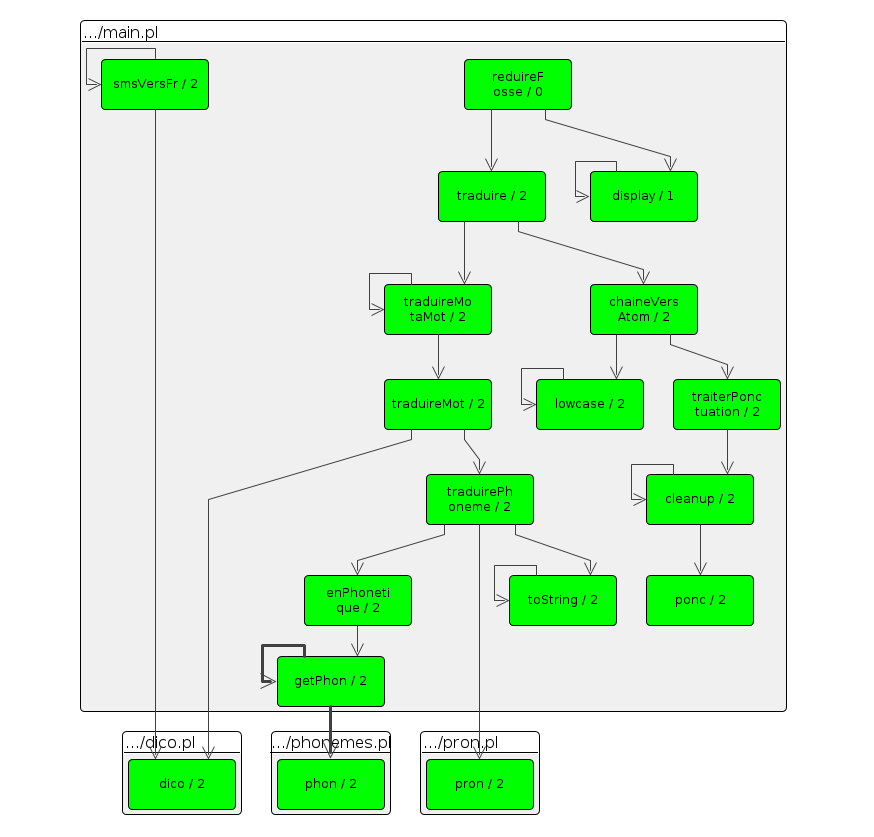
\includegraphics[scale=0.60]{mainpl.png}
	\end{figure}
 
\chapter{Conclusion}
	\section{A vous de jouer}
	Bien, vous savez désormais comment fonctionne la traduction, mais vous aimeriez surtout traduire le message mystérieux envoyé par votre neveu. Pour cela, il faut télécharger SWI-Prolog\footnote{http://www.swi-prolog.org/download/stable} puis ouvrir la console SWI-Prolog ( {\em swipl} sous GNU/Linux ) et consulter le fichier de projet. Pour cela écrivez juste {\em [/chemin/vers/le/fichier/main].} ( à noter qu'il ne faut pas rajouter l'extension de fichier {\em .pl} dans le chemin ). Le fichier main.pl s'occupera de charger tous les autres fichiers nécessaires. Une fois ceci fait, vous pouvez utiliser les règles {\em reduireFosse/0} et {\em traduire/2} comme vu précédemment.\\
	Voila ! A vous de jouer !
	
	\section{Les insectes attaques !}
	Aucun problème n'est parfait, le notre n’échappe pas non plus à quelques bugs. Si l'utilisation de Prolog qui est un langage haut niveau permet de se soustraire des bugs techniques, il réside certains défauts :\\
	La traduction par phonétique est très dépendante de son dictionnaire, hors, dû à l'irrégularité de la syntaxe Wikipedia, le fichier de dictionnaire a été grossièrement parsé et possède de nombreux bugs ( par exemple, à un moment, {\em "sha"} était traduit par {\em "phytotoxique"} car une erreur de parsage avait donné à ce dernier la phonétique "\textipa{\:la}" ).\\
	De plus, notre algorithme de traduction vers la phonétique est souvent erroné dû au fait que les phonèmes du français ne sont pas toujours exactement utilisés dans le SMS ce qui résulte en des erreurs de traduction.\\
	La traduction est donc encore loin d'être parfaite et nécessite encore des améliorations. 
	
	\section{Voyons plus grand ! Voyons plus loin !}
	Et bien, puisque nous parlions d'améliorations, voyons un peu celle que, si nous avions eu plus de temps, nous aurions pu apporter.\\
	Tout d'abord, pour améliorer la traduction, nous aurions pu utiliser un {\em modèle de langue}. C'est une méthode statistique qui permet de déterminer les régularités d'un langage. En d'autre terme, nous aurions pu déterminer la probabilité de la traduction d'un mot en fonction des mots qui l'entoure.\\
	Une autre amélioration qui n'a pas de rapport avec la traduction est celle de créer une GUI. SWI-Prolog permet d'embarquer son interpréteur dans de nombreux langages, dont Java. Nous aurions donc pu très bien imaginer une application Android\footnote{https://fr.wikipedia.org/wiki/Android} qui aurait permis à l'utilisateur de traduire simplement les SMS qu'il reçoit.
	
	\section{Credit ( Non ce n'est pas de l'argent )}
	Avant de finir ce rapport, nous tenons à remercier plusieurs organisations et personnes pour l'aide, directe ou indirecte, qu'ils nous ont apporté :
	\begin{itemize}
		\item Monsieur Nicolas Hernandez, notre professeur encadrant pour l'aide et les conseils qu'il nous a apporté.
		\item La fondation Wikimedia sans qui nous n'aurions pu obtenir simplement la liste des phonèmes Français et un dictionnaire phonétique. A ce titre, et au tire de la licence GFDL, tout crédit leur revient pour les fichiers phonemes.pl et pron.pl.
		\item Alain Colmerauer, Philippe Roussel et toute autre personne ayant participé à la conception de Prolog, sans quoi ce projet n'aurait jamais existé.
		\item Jan Wielemaker et tous les contributeurs à SWI-Prolog pour avoir créé un interpréteur Prolog sous licence libre extrêmement puissant.
		\item  Patrick Blackburn, Johan Bos, et Kristina Striegnitz pour leurs cours sur Prolog {\em "Learn Prolog Now !}\footnote{http://www.learnprolognow.org/} qui nous aura aidé durant notre apprentissage de Prolog.
		\item Et finalement, Emmanuel Adam pour ses cours et exercices Prolog.
	\end{itemize}
	
	\newpage
	
	\begin{center}
		\Huge Rapport de Projet Technologique\\
		\bigskip 
		\bigskip 
		\bigskip 
		\bigskip 
		\LARGE Université de Nantes\\ Institut Universitaire de Technologie\\ Département Informatique
	\end{center}

\end{document}
